% TeX eps-loader file generated by PosteriorIRF.m (Dynare).
% 31-Jan-2024 13:28:51
 
\begin{figure}[H]
\centering 
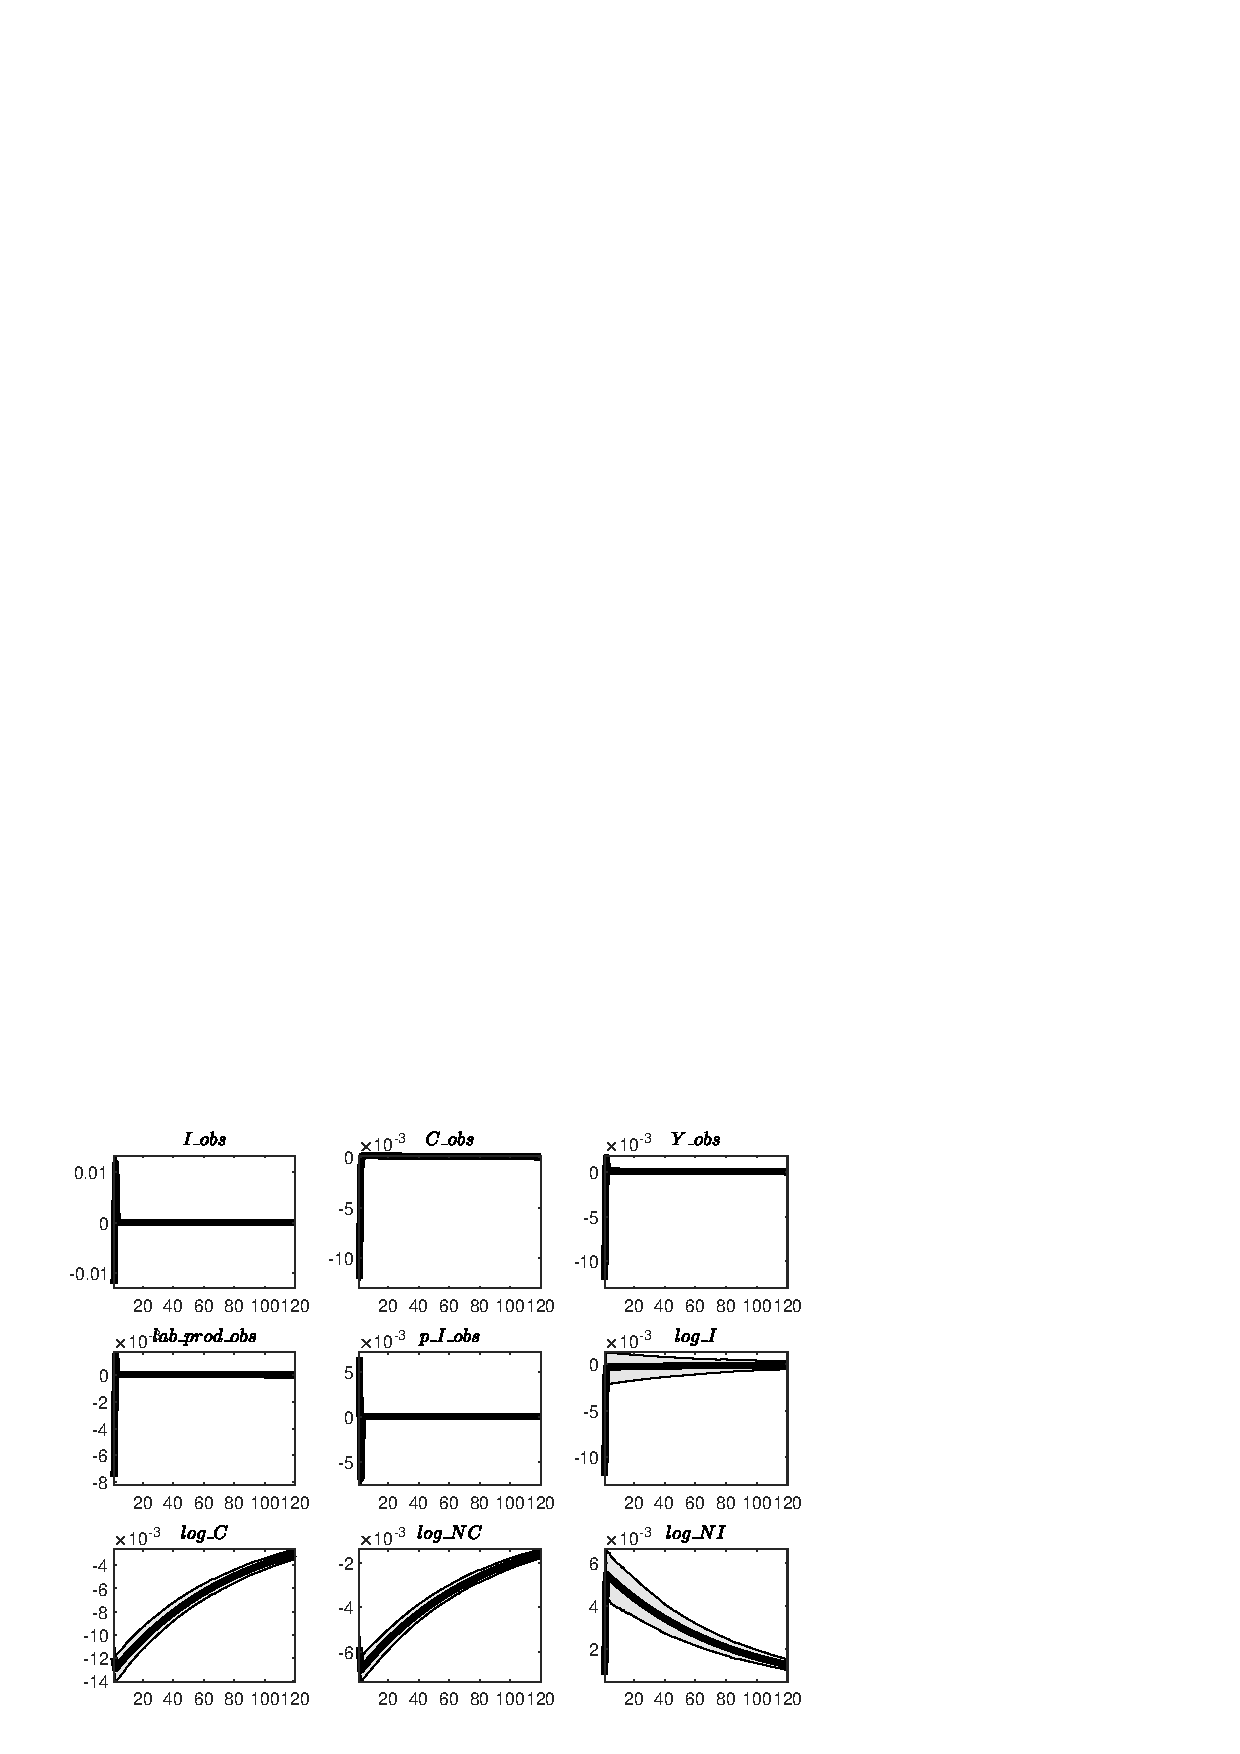
\includegraphics[width=0.80\textwidth]{BRS_growth_ext_comovement/Output/BRS_growth_ext_comovement_Bayesian_IRF_e_g_1}
\caption{Bayesian IRF: Orthogonalized shock to ${e_g}$.}
\label{Fig:BayesianIRF:e_g:1}
\end{figure}
 
\begin{figure}[H]
\centering 
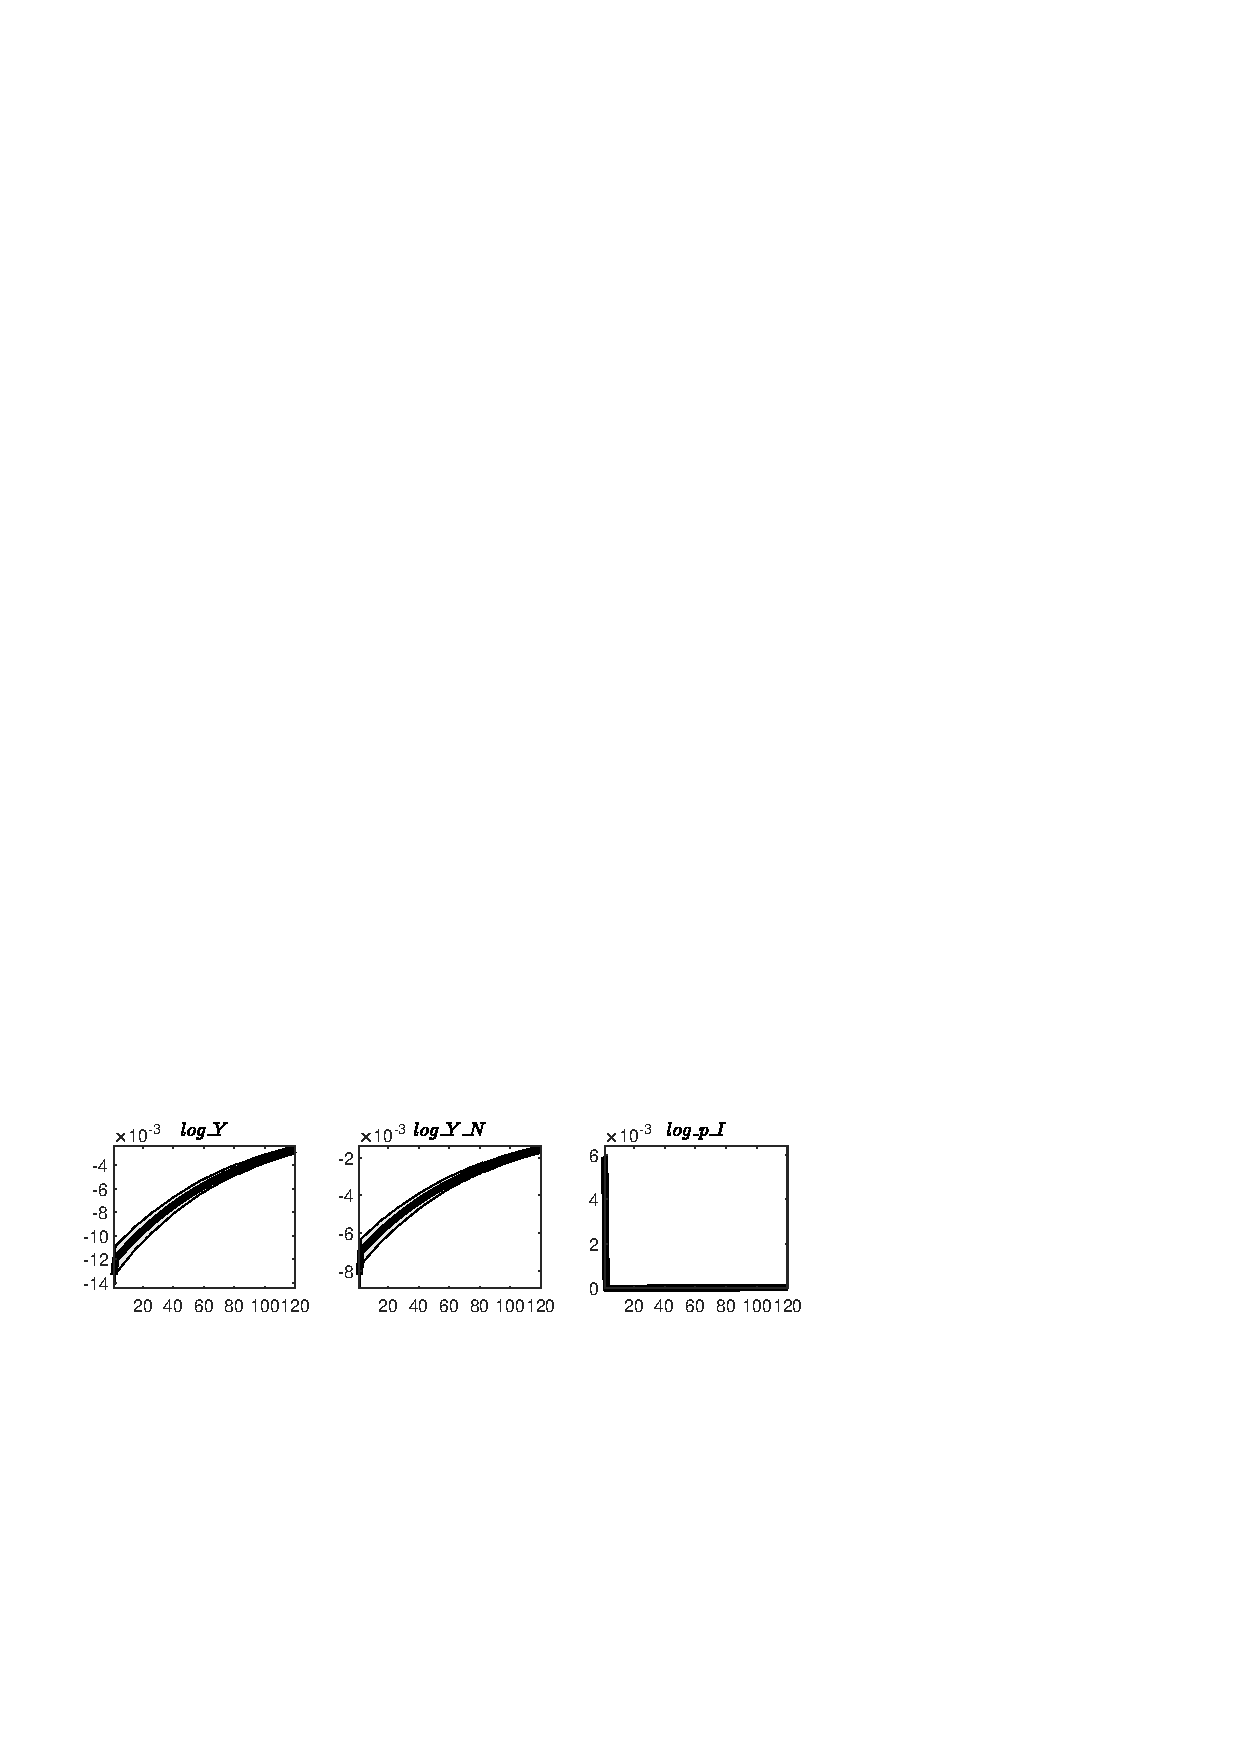
\includegraphics[width=0.80\textwidth]{BRS_growth_ext_comovement/Output/BRS_growth_ext_comovement_Bayesian_IRF_e_g_2}
\caption{Bayesian IRF: Orthogonalized shock to ${e_g}$.}
\label{Fig:BayesianIRF:e_g:2}
\end{figure}
 
\begin{figure}[H]
\centering 
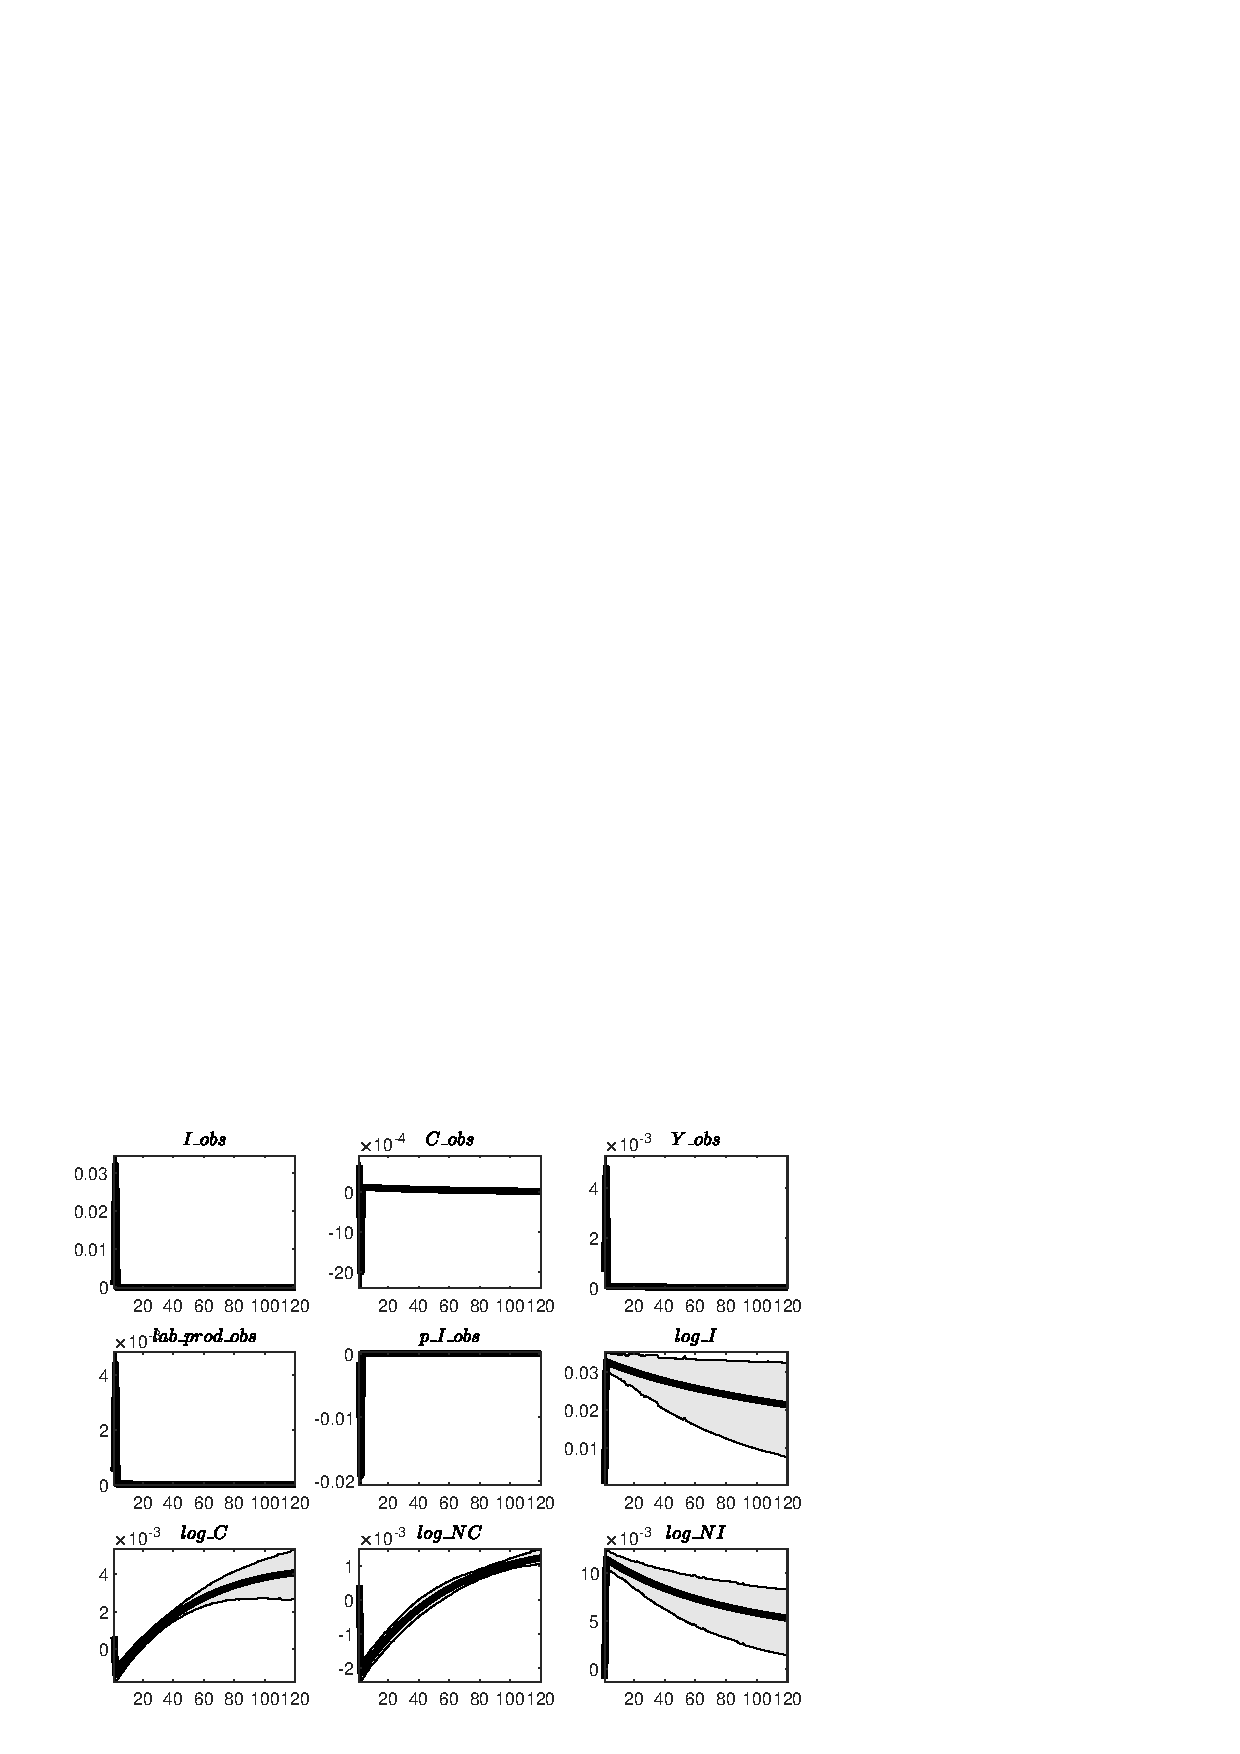
\includegraphics[width=0.80\textwidth]{BRS_growth_ext_comovement/Output/BRS_growth_ext_comovement_Bayesian_IRF_e_ZI_1}
\caption{Bayesian IRF: Orthogonalized shock to ${e_{ZI}}$.}
\label{Fig:BayesianIRF:e_ZI:1}
\end{figure}
 
\begin{figure}[H]
\centering 
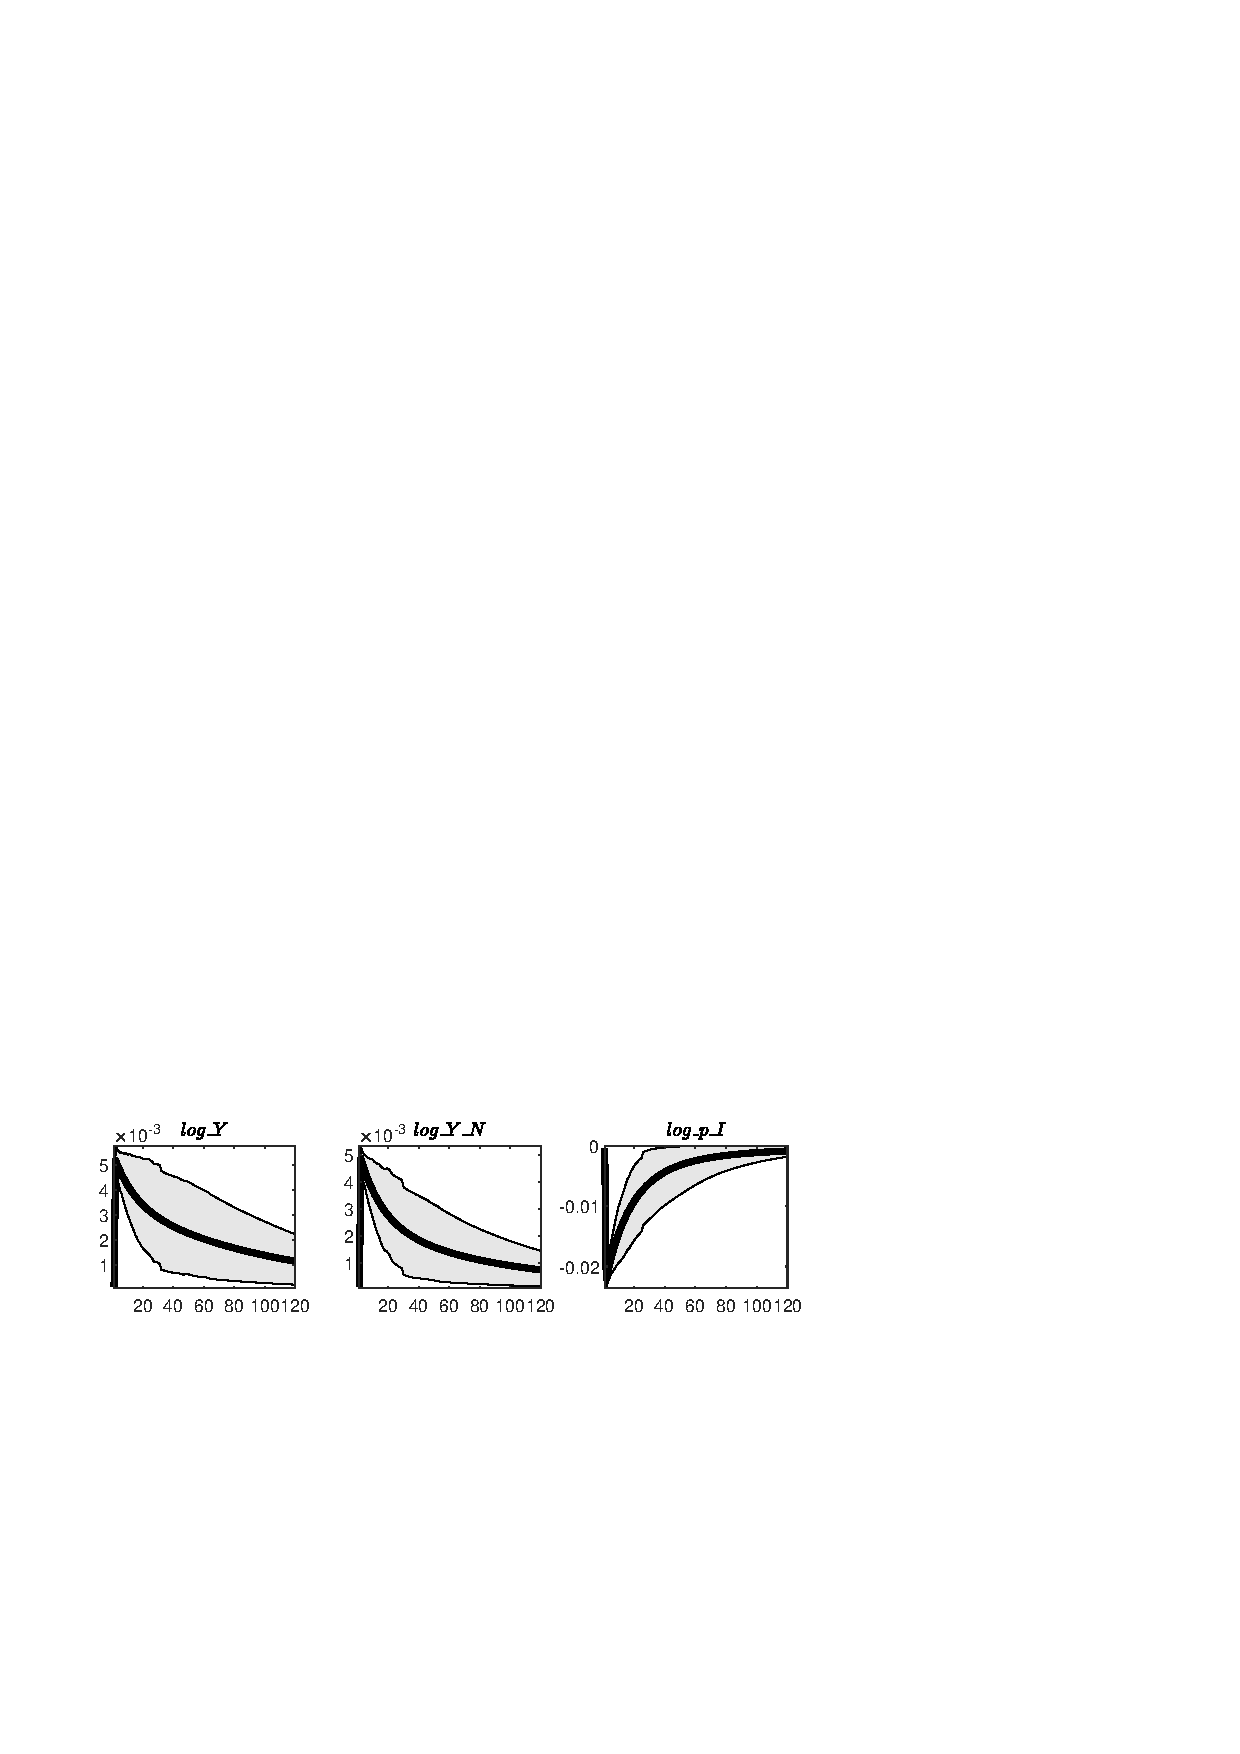
\includegraphics[width=0.80\textwidth]{BRS_growth_ext_comovement/Output/BRS_growth_ext_comovement_Bayesian_IRF_e_ZI_2}
\caption{Bayesian IRF: Orthogonalized shock to ${e_{ZI}}$.}
\label{Fig:BayesianIRF:e_ZI:2}
\end{figure}
 
\begin{figure}[H]
\centering 
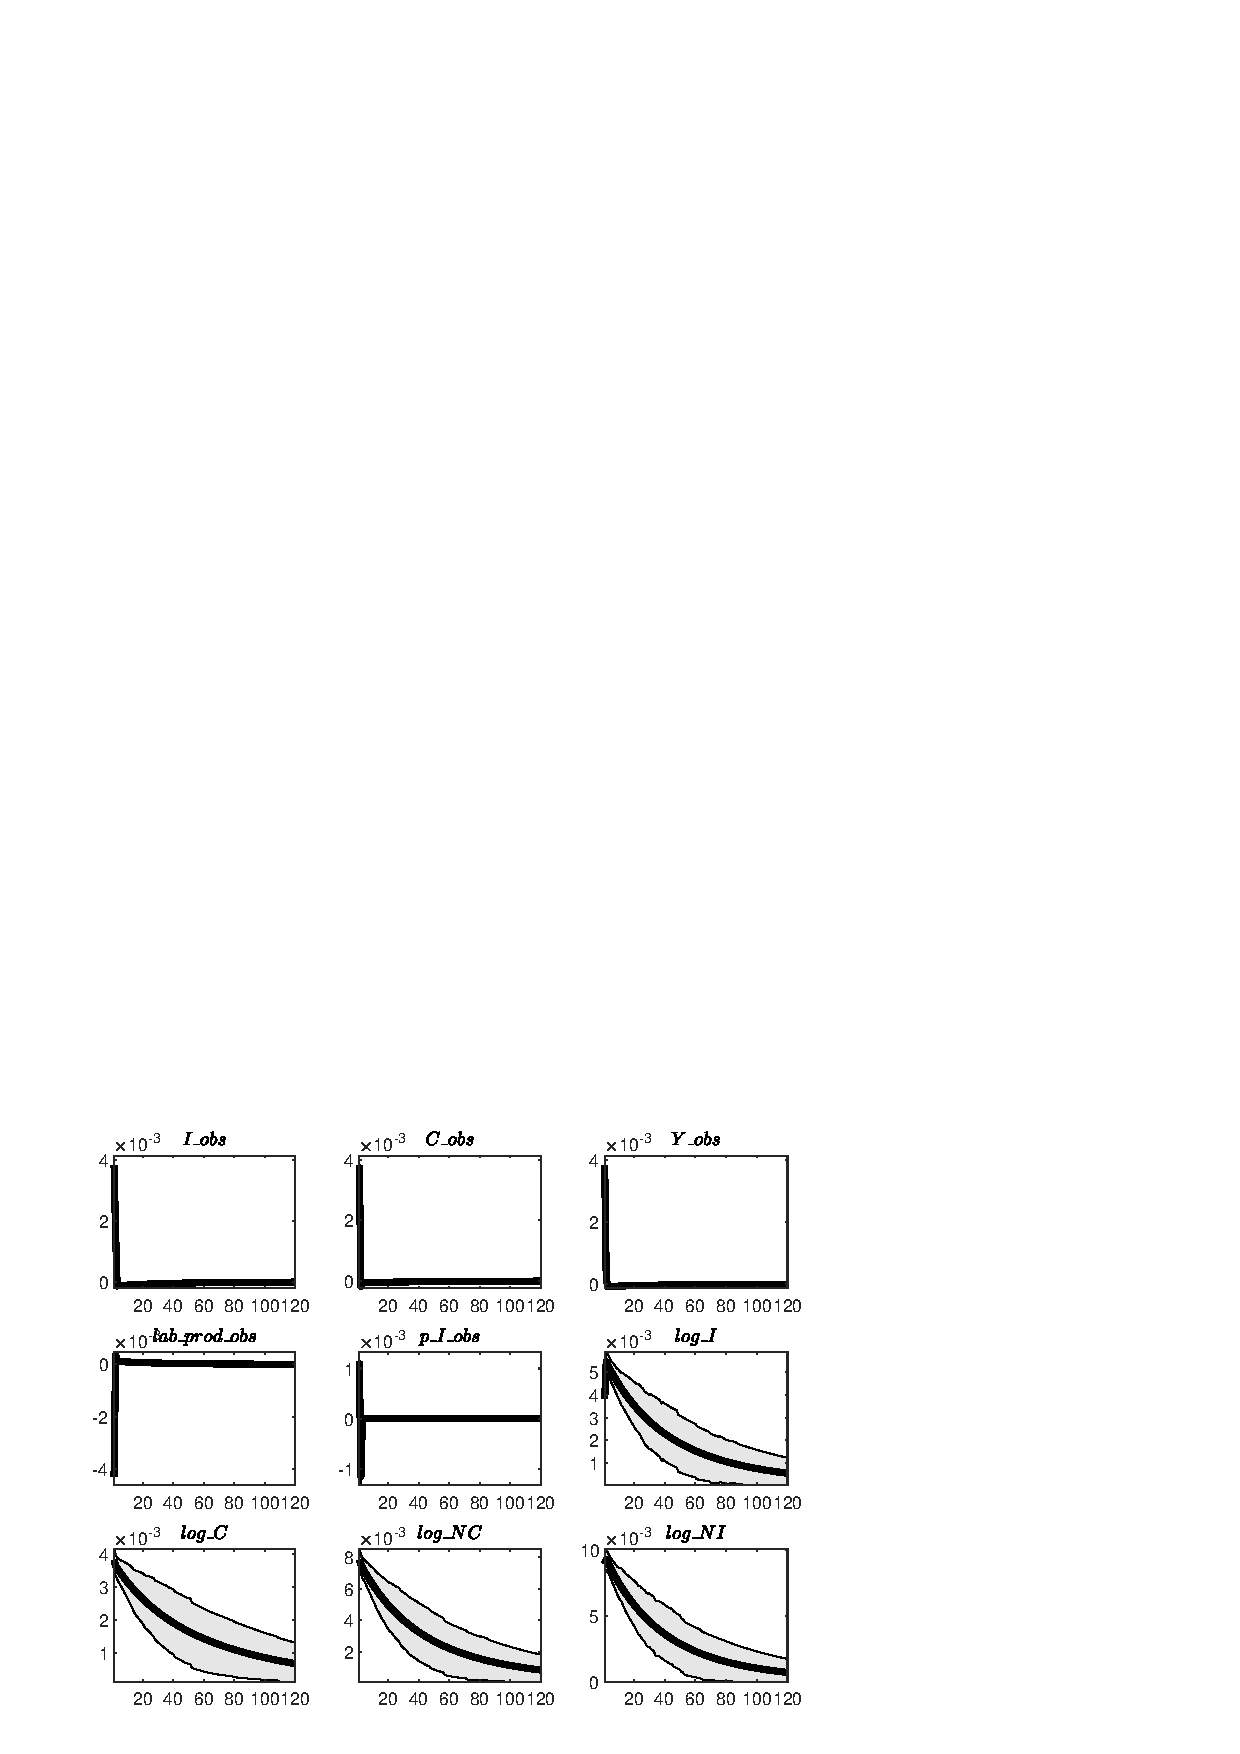
\includegraphics[width=0.80\textwidth]{BRS_growth_ext_comovement/Output/BRS_growth_ext_comovement_Bayesian_IRF_e_N_1}
\caption{Bayesian IRF: Orthogonalized shock to ${e_N}$.}
\label{Fig:BayesianIRF:e_N:1}
\end{figure}
 
\begin{figure}[H]
\centering 
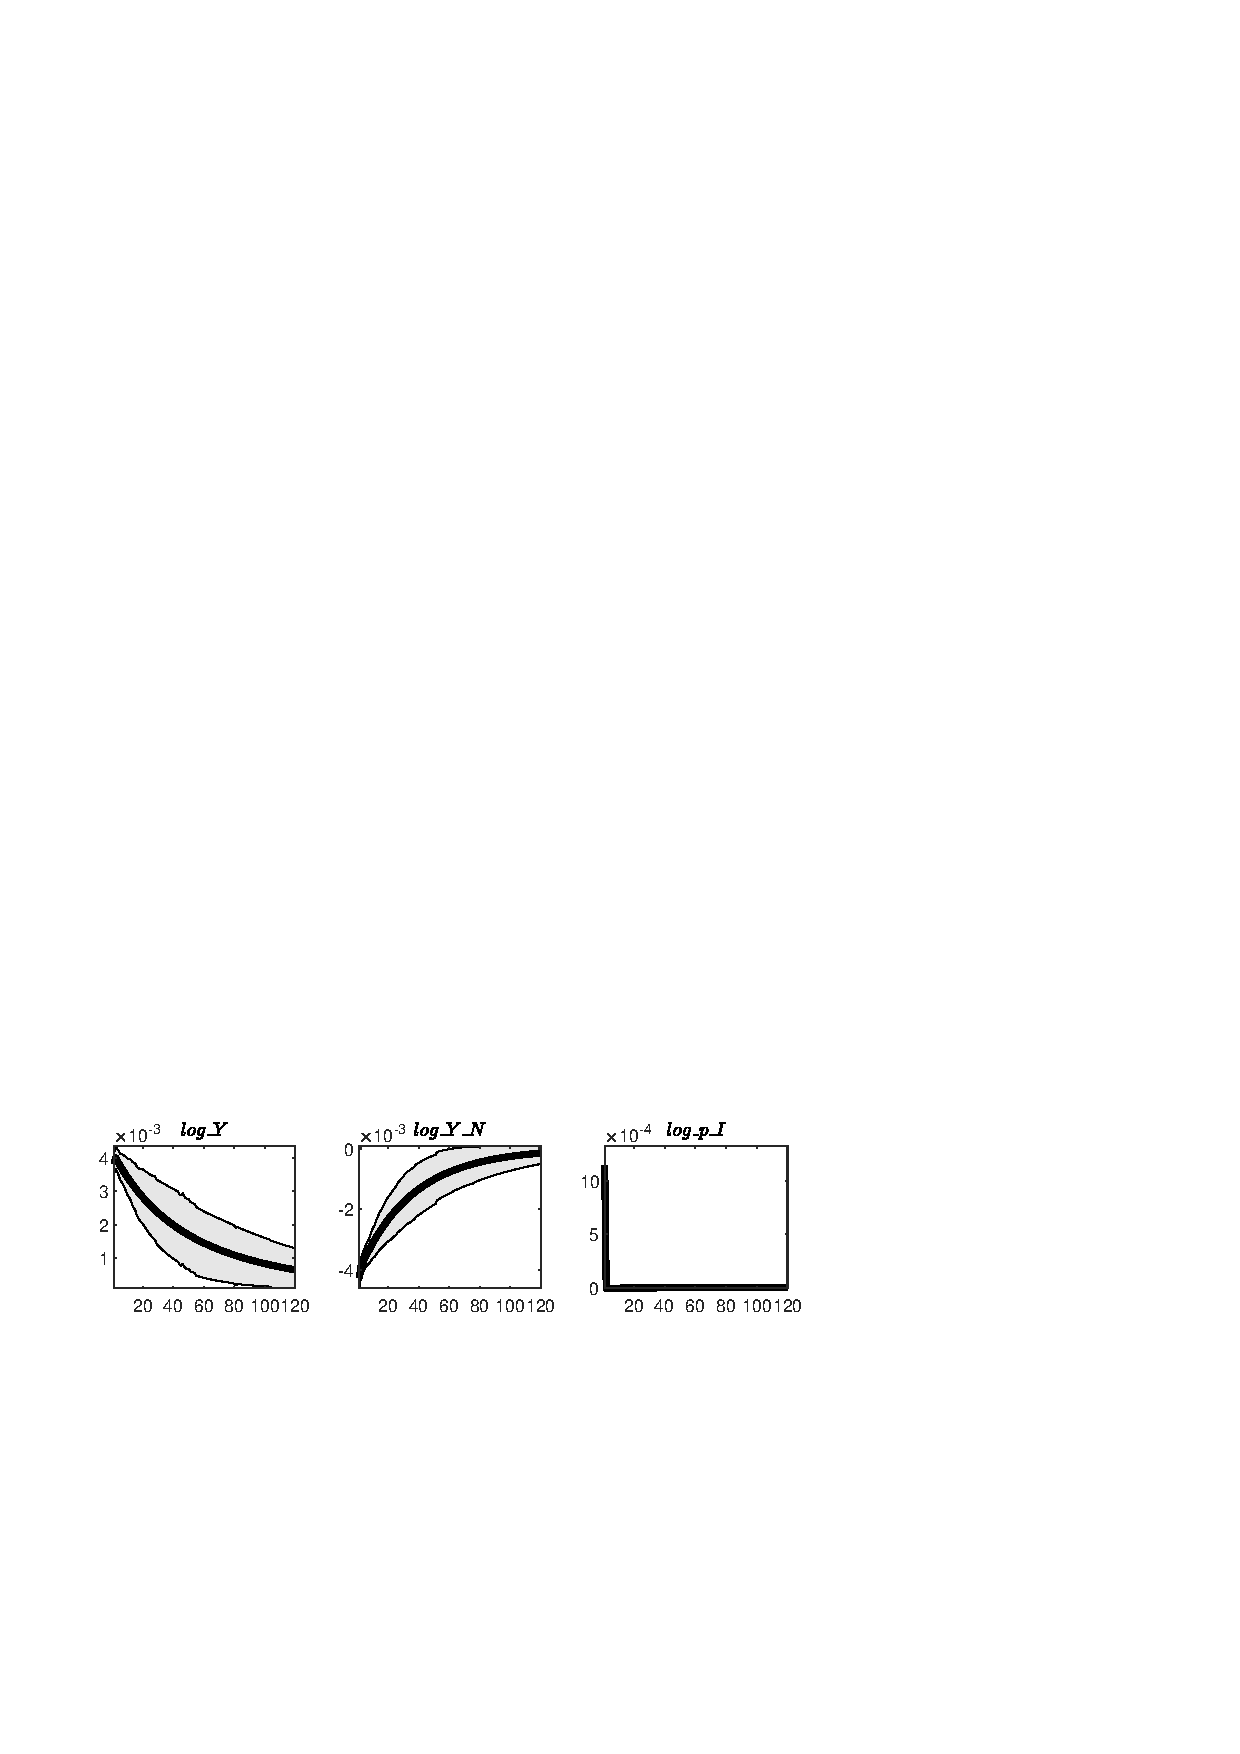
\includegraphics[width=0.80\textwidth]{BRS_growth_ext_comovement/Output/BRS_growth_ext_comovement_Bayesian_IRF_e_N_2}
\caption{Bayesian IRF: Orthogonalized shock to ${e_N}$.}
\label{Fig:BayesianIRF:e_N:2}
\end{figure}
 
\begin{figure}[H]
\centering 
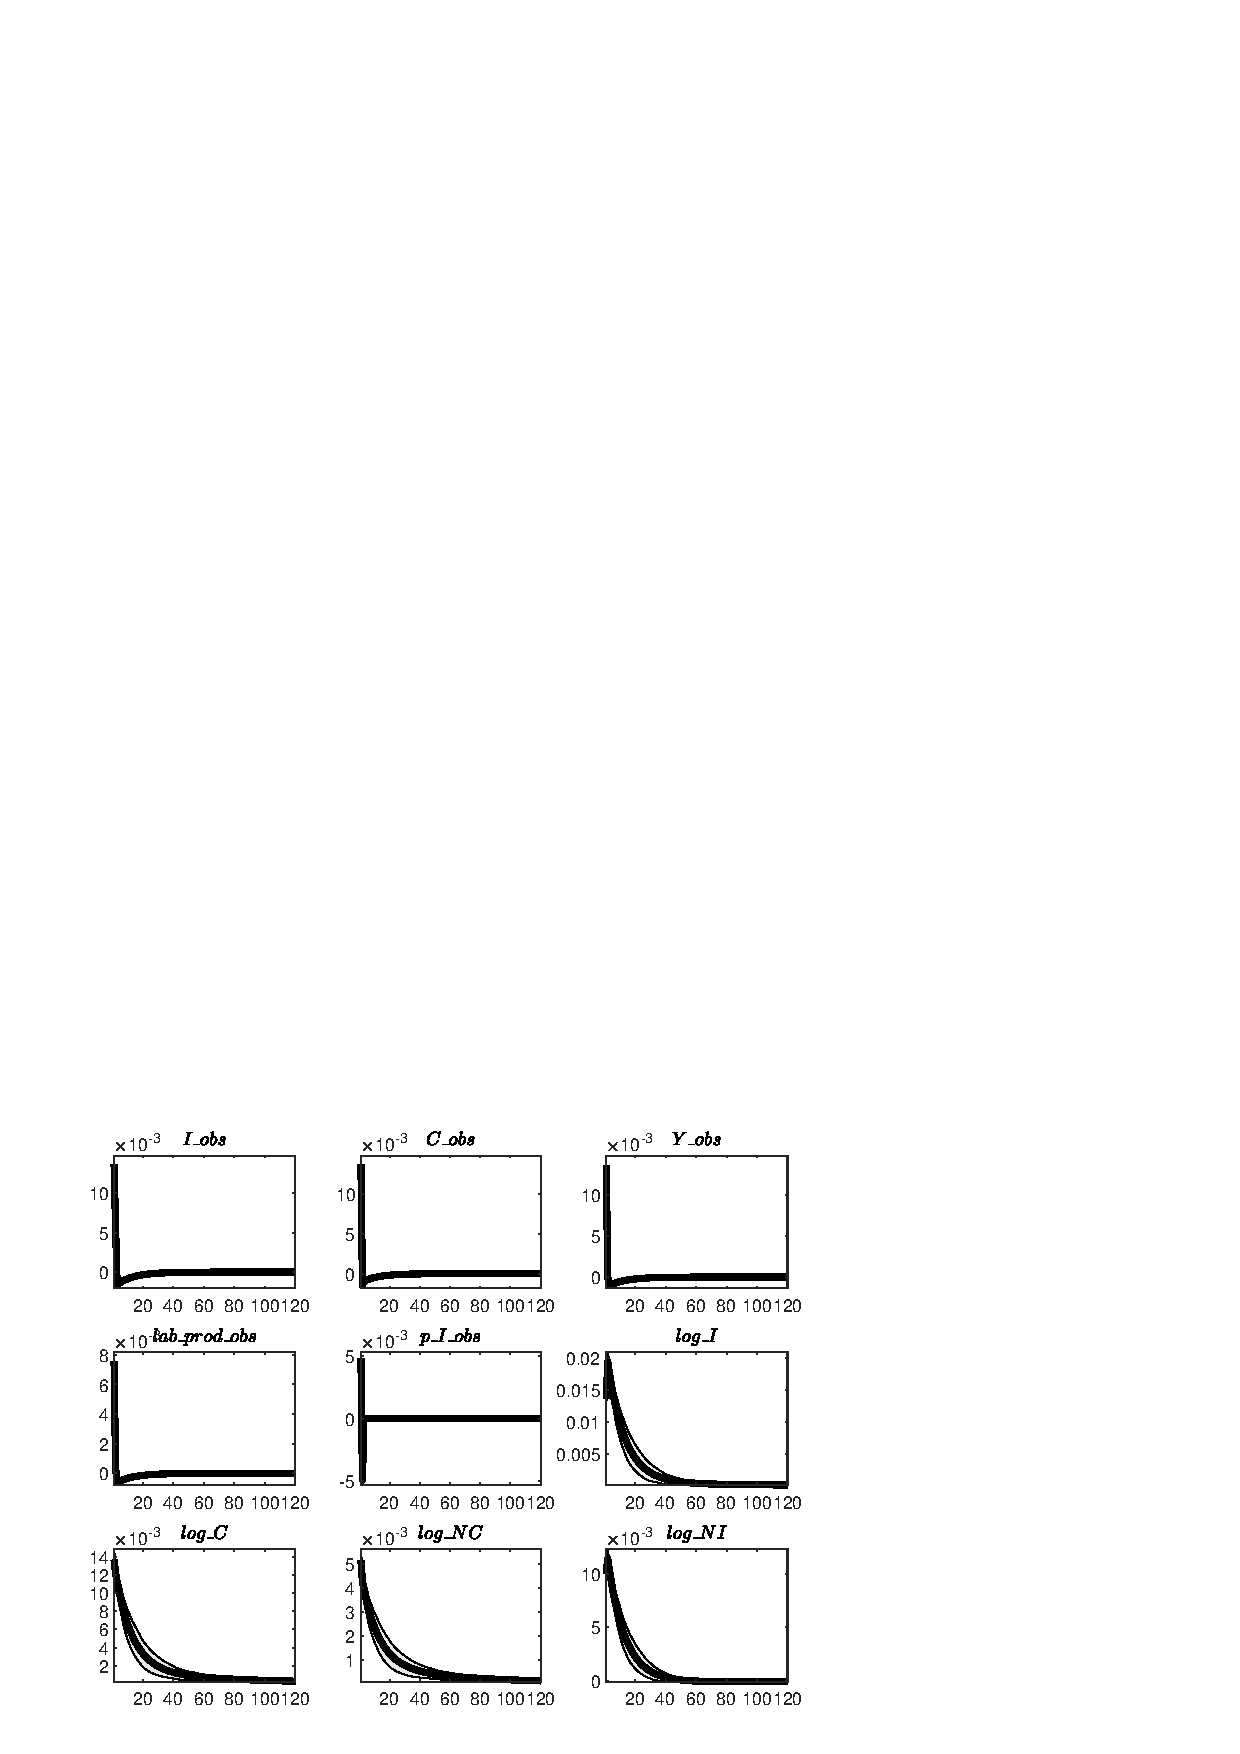
\includegraphics[width=0.80\textwidth]{BRS_growth_ext_comovement/Output/BRS_growth_ext_comovement_Bayesian_IRF_e_D_1}
\caption{Bayesian IRF: Orthogonalized shock to ${e_D}$.}
\label{Fig:BayesianIRF:e_D:1}
\end{figure}
 
\begin{figure}[H]
\centering 
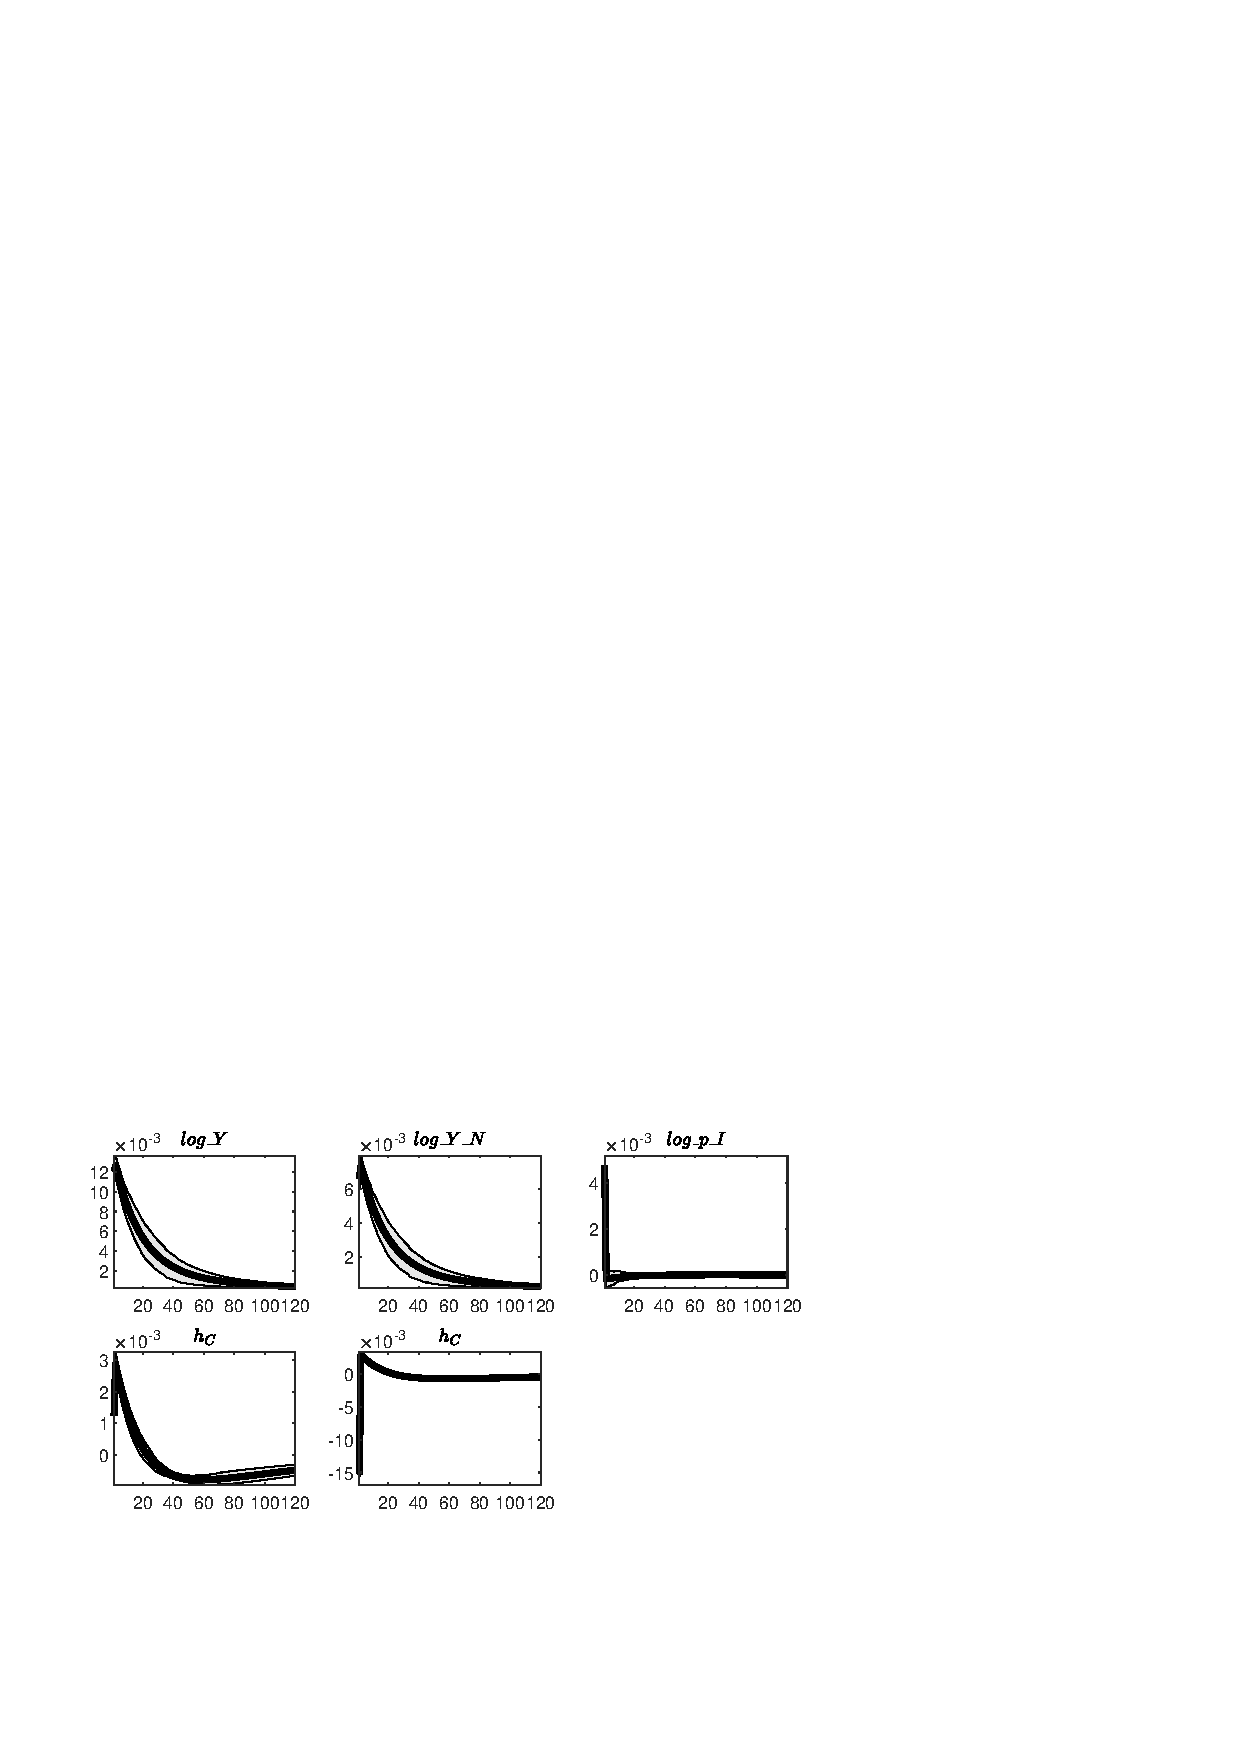
\includegraphics[width=0.80\textwidth]{BRS_growth_ext_comovement/Output/BRS_growth_ext_comovement_Bayesian_IRF_e_D_2}
\caption{Bayesian IRF: Orthogonalized shock to ${e_D}$.}
\label{Fig:BayesianIRF:e_D:2}
\end{figure}
 
% End of TeX file.
